\documentclass[../main.tex]{subfiles}
\begin{document}
\paragraph{Offline solutions}\label{par:poisson_fom}

Following the SVD, during the offline stage, we observe that $N_{r}=2$ according to Definition \ref{def:kolmogoroff_n_width}, meaning that we only need $2$ basis functions to retain $99\%$ of the accuracy of the FOM.
In Figure \ref{fig:poisson_fom} we report the high-order solutions computed at offline phase for the parameter values $P=\{\mu\in\mathcal{P}\;:\;\mu = 0.1 + n\frac{0.9}{N_{f}}\,,\;n=1,\dots,N_{f}\}\subset\mathcal{P}$.

\begin{figure}[H]
    \centering 
    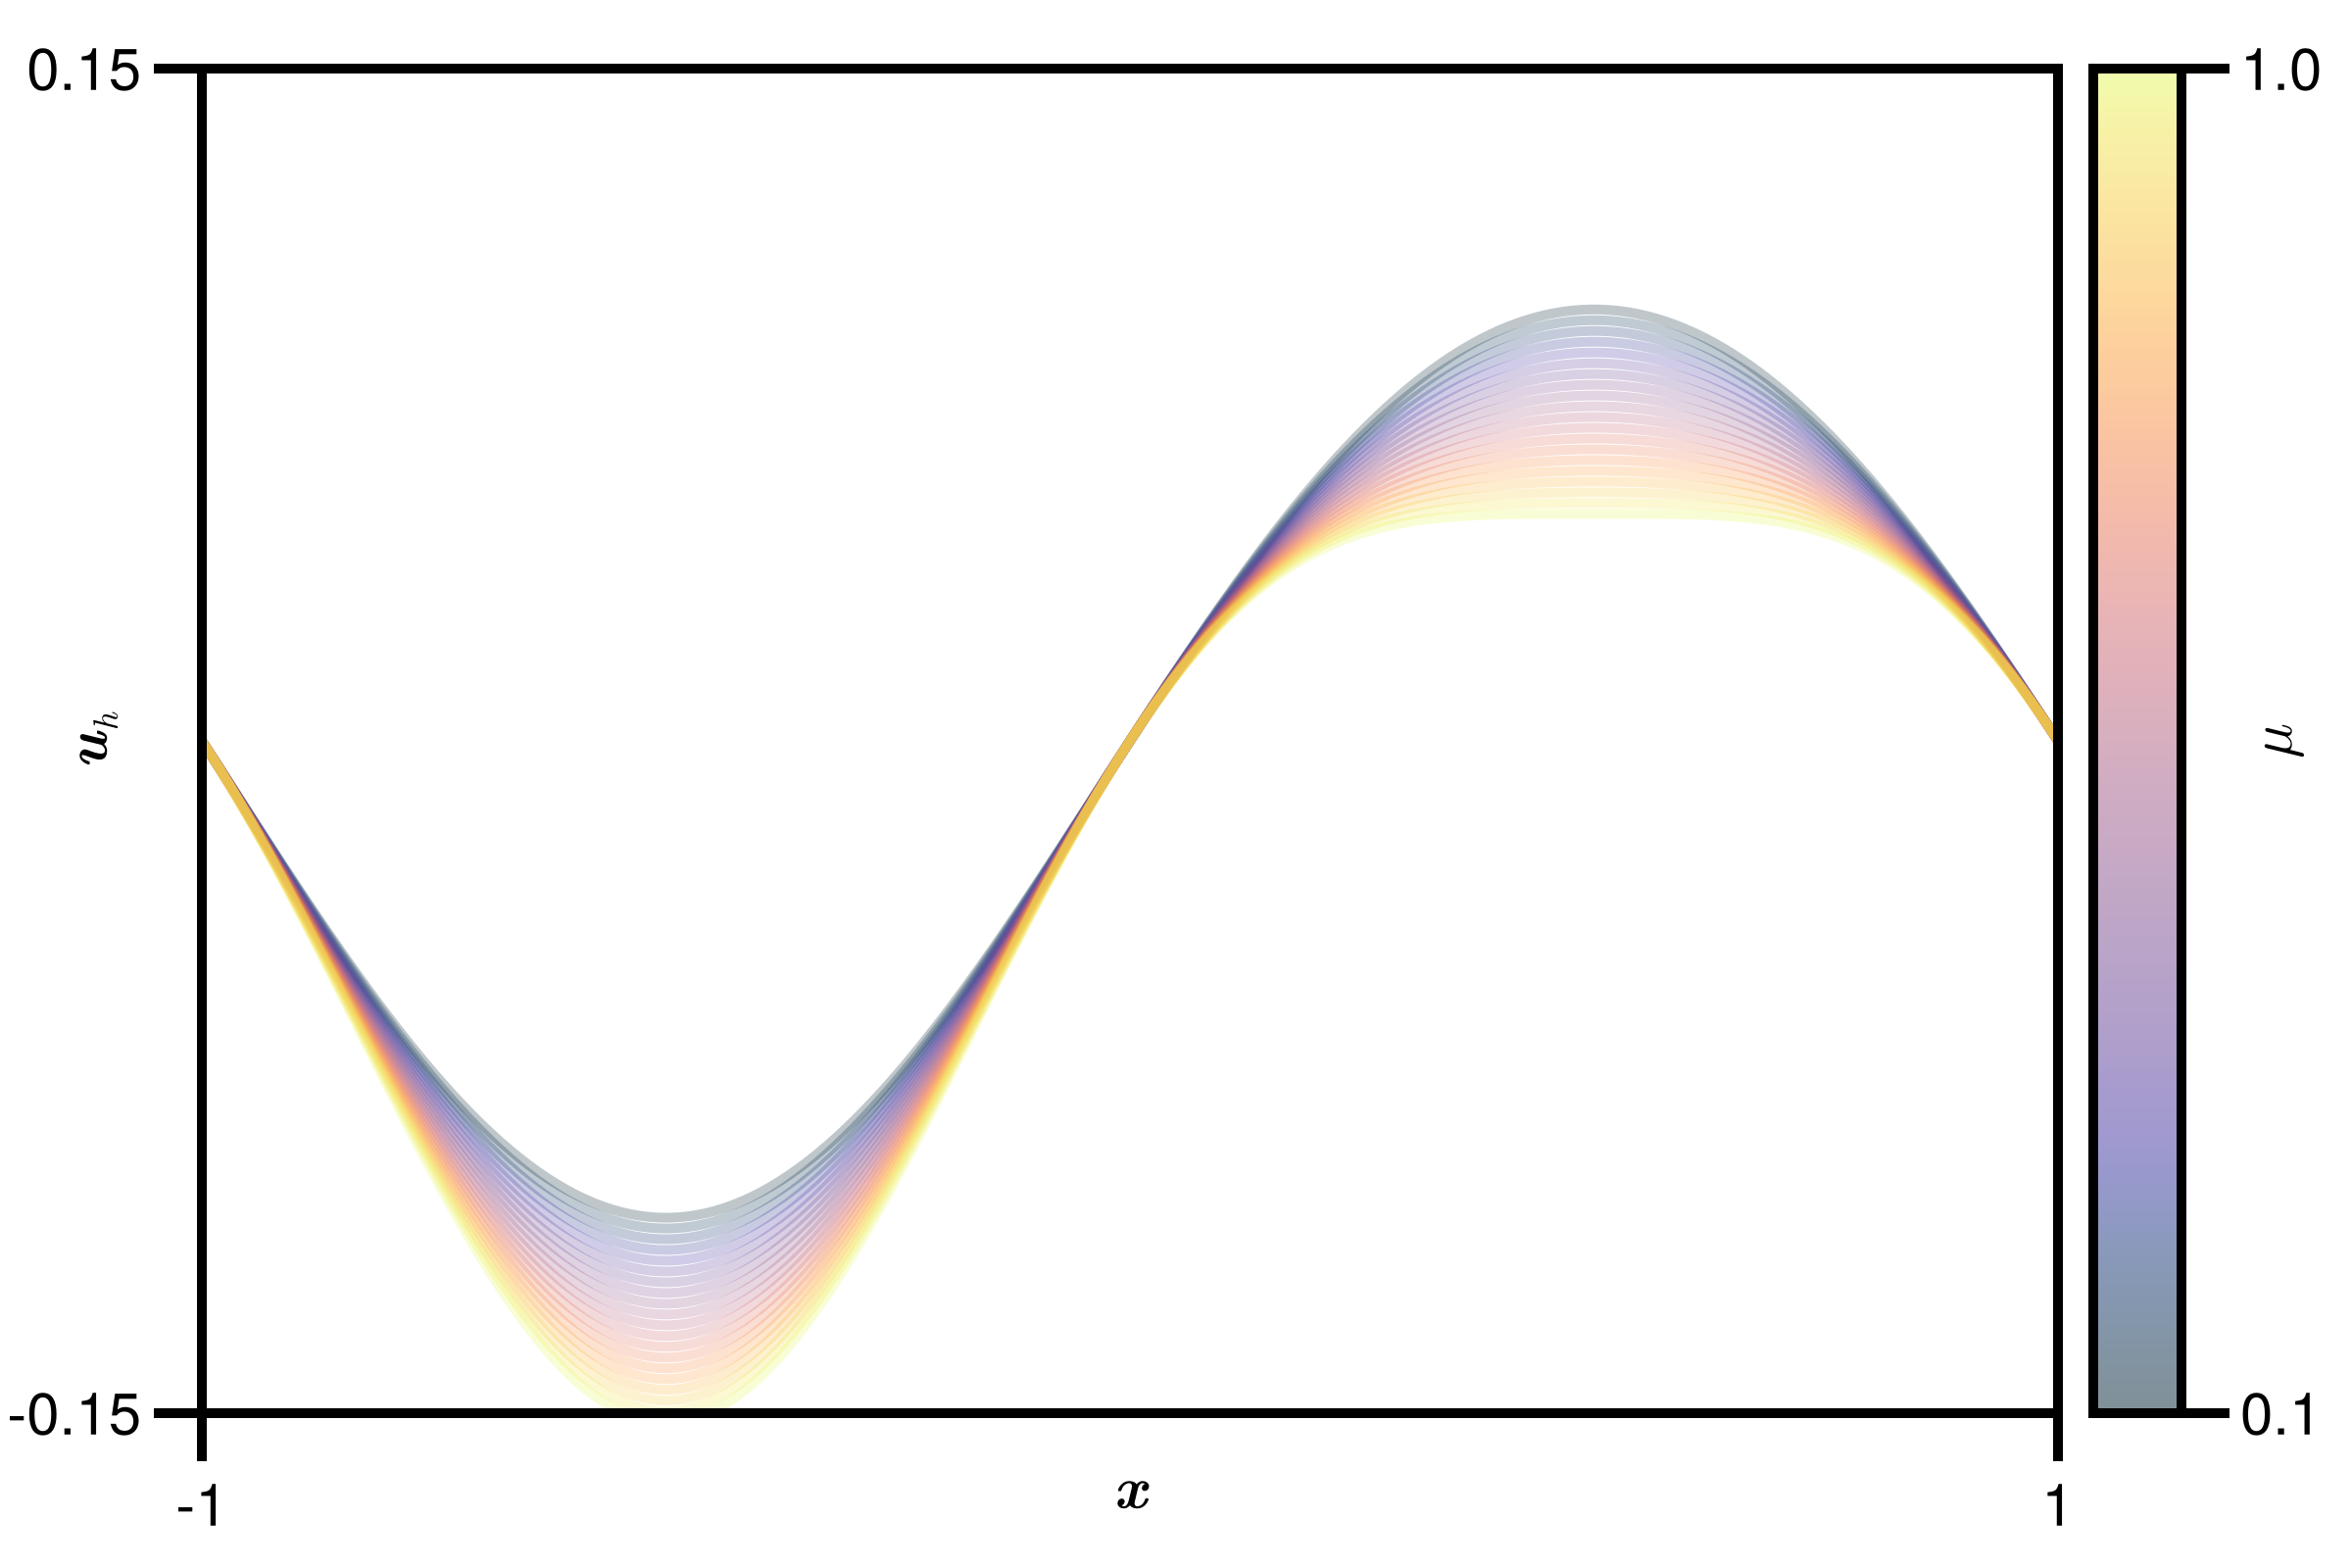
\includegraphics[keepaspectratio, width=0.7\textwidth]{../figures/fig:poisson_fom.png}
    \caption{Solutions/snapshots of the FOM of \eqref{eq:poisson} at different parameter values.}
    \label{fig:poisson_fom}
\end{figure}

\end{document}
